% !TeX spellcheck = en_US
\chapter{Introduction}

\ac{AI} is the study field that leverages the ability of machines to mimic the problem-solving skill of human. In other words, \ac{AI} pushing machines to think, act like people, in a rational way. It lies in the core of countless novel applications in real life, self-driving cars, virtual assistant, face recognition, \etc. \ac{ML} is a sub-field of \ac{CS} and \ac{AI}, that “gives computers the ability to learn without being explicitly programmed” (\href{https://en.wikipedia.org/wiki/Machine_learning}{Wikipedia}). As a great amount of collected data and powerful computational hardware arise, \ac{DL} is then a subset of \ac{ML} (\figref{fig:relation-ai-ml-dl}). Advanced applications which relate to \ac{NLP}, \ac{CV}, robotic learning, \etc, are with in this \ac{DL} subset.
\begin{figure}[hbt!]
	\centering
	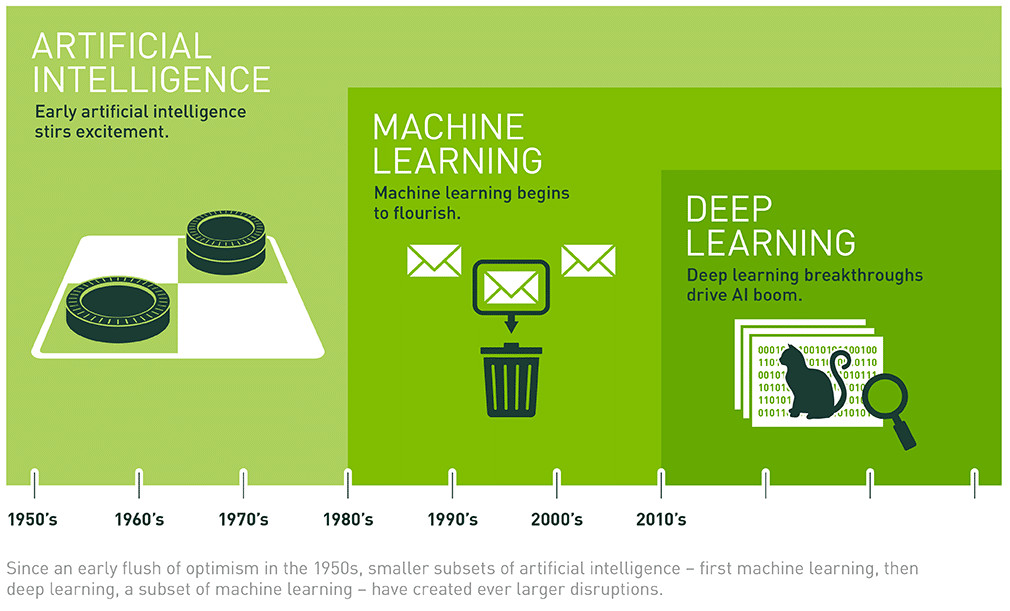
\includegraphics[width=1\textwidth]{nvidia-ai-ml-dl.jpg}
	\caption{The relation between \ac{AI}, \ac{ML} and \ac{DL} (\href{https://developer.nvidia.com/deep-learning}{src}).}
	\label{fig:relation-ai-ml-dl}
\end{figure}

It's important to understand that there are more to \ac{AI} and \ac{ML} than just neural networks. In the end, to create a meaningful and working neural network, one should have strong background in the basics of \ac{ML} as well.

These notes are my way of keeping record of what I have learn in the field. The structure of the notes is as follows:
\begin{itemize}
	\item \charef{cha:overview-ml} introduces common ideas in \ac{ML}.
	\item \charef{cha:probabilities} presents the mathematics background on probabilities, matrix.
	\item \todo{chapter 3} explain basic concepts, the branching of different classes in \ac{ML}. Later chapters presents each smaller branches.
\end{itemize}

\todo{The structure of the notes}